\documentclass[preprint2,numberedappendix,tighten,twocolappendix]{aastex6}
\shorttitle{ECHO}
\shortauthors{Jacobs, et. al.}

\usepackage{amsmath}
\usepackage{graphicx}
\usepackage[figuresright]{rotating}
\usepackage{natbib}
\usepackage{ctable}
\usepackage{tabularx}
\usepackage{enumitem}
\usepackage{url}
\setlist[itemize]{noitemsep, topsep=0pt}
\setlist[enumerate]{noitemsep, topsep=0pt}
\citestyle{aa}



\begin{document}


\title{The External Calibrator for Hydrogen Observatories}



\author{
Daniel C. Jacobs\altaffilmark{1},
Jacob Burba\altaffilmark{1},
Judd Bowman\altaffilmark{1},
Lauren Turner\altaffilmark{1}
}


\affiliation{1}{School of Earth and Space Exploration, Arizona State U., Tempe, AZ, 85287}


\begin{abstract}
We describe the External Calibrator for Hydrogen Observatories (ECHO)
\end{abstract}




\section{Introduction}\label{sec:intro}

A new generation of radio arrays is being developed that use large numbers of low-cost elements, such as phased tiles of dipole antennas. This is made possible by developments in digital technology and enables exploration of new windows on the universe such as the epoch of reionization (EoR) via the redshifted 21 cm line \citep{Morales:2010p8093,Furlanetto:2006p2267,Madau:1997p2232}. Precise calibration of the primary beams of these dipole arrays has been found to be crucial to analysis of observations by widefield radio arrays such as the MWA \citep{Tingay:2013p9022,Bowman:2013p9950}, PAPER \citep{Pober:2012p8800,2015ApJ...809...61A,2013ApJ...776..108J}, LOFAR \cite{Yatawatta:2013p9699}, HERA \citep{2016:deBoerHERAarxiv} and SKA-low \citep{Mellema:2013p10035,Mort:2016SKAlowimagingarxiv}.

The chief challenge in observing highly redshifted 21\,cm is discriminating the mK level spectral line signal against the $\sim$100K foregrounds.  Instrumental simulations have found that bright sources far from the pointing center, though attenuated significantly by the beam, introduce foreground signals which are highly chromatic and difficult to discriminate from the cosmological 21cm spectral line signature \citep{Thyagarajan:2013p10039,2015ApJ...804...14T,Mort:2016SKAlowimagingarxiv}. These effects have been confirmed in both MWA and PAPER observations \citep{2015:ThyagarajanConfirmationwidefield,Pober:2016ApJ...819....8P}. Precision removal of foreground sources far into the sidelobes is one of the chief challenges of the primary analysis pipelines  \citep{2016:JacobsPipelinepaper} however the amount which can be removed is limited by the accuracy of our knowledge of the antenna response.  More detailed electromagnetic models have been shown to improve the overall accuracy of flux reconstruction \citep{Sutinjo:2015RaSc...50...52S}. however a single digital model cannot account for as-built variation which has been shown to be significant and largely unavoidable without large added expense \citep{2016:NebenBeamformingerrors}.  The largest success of improved modeling accuracy has been in improving polarization response. Polarization signals have inherent spectral variation due to faraday rotation imprinted by magnetized ionized plasmas in the interstellar medium as well as the ionosphere. Leakage of these spectral signatures into the unpolarized reionization signal can be minimized with a combination of beam modeling and careful element design \citep{Jelic:2010p8293,Moore:2013p9941,Asad:2015LofarPol}. Another feature of cosmological distance 21cm observations is the wide spectral bandwidth, at least 100 to 200 MHz to span a useful redshift range. Successful foreground isolation across this range necessitates knowledge of the beam response across this entire range.  Spectral variation of the beam has been found to cause otherwise smooth foregrounds to contribute an additional foreground component\citep{2016:ThyagarajanBeamChromaticity,2016:EwallWiceHERAdisharXiv}. An inaccurate beam model also limits the accuracy of calibration. The usual solution is to only use calibration sources in the well known parts of the beam, however incomplete foreground models have been shown to lead to spectral line foregrounds \citep{2016:BarryCalibrationRequirements}.  Calibration error is not just limited to sky modeling. Arrays such as PAPER and HERA are taking advantage of baseline redundancy to calibrate without sky models \citep{Liu:2010p10391,Zheng:2014p10467,2015ApJ...809...61A}, however this technique is subject to error due to deviations from redundancy caused by beam variation from antenna to antenna. Though more work is necessary to understand the impact of beam non-redundancy, its clear that more needs to be known about the actual as-built variation.  Accurate knowledge of the beam can dramatically improve the quality of analysis steps but is also key information during the design process as a validation of modeling and to explore design choices \citep{2014IAWPL..13..169V,2016:NebenHERAdish}.

Taken together, we can summarize the reionization needs for beam measurements as:
\begin{itemize}
\item precision at the horizon as good as the phase center
\item sampling across the desired bandwidth
\item full polarization sampling
\item maps of the in-situ / as-built antennas
\end{itemize} 


\begin{figure*}[htb]
\centering
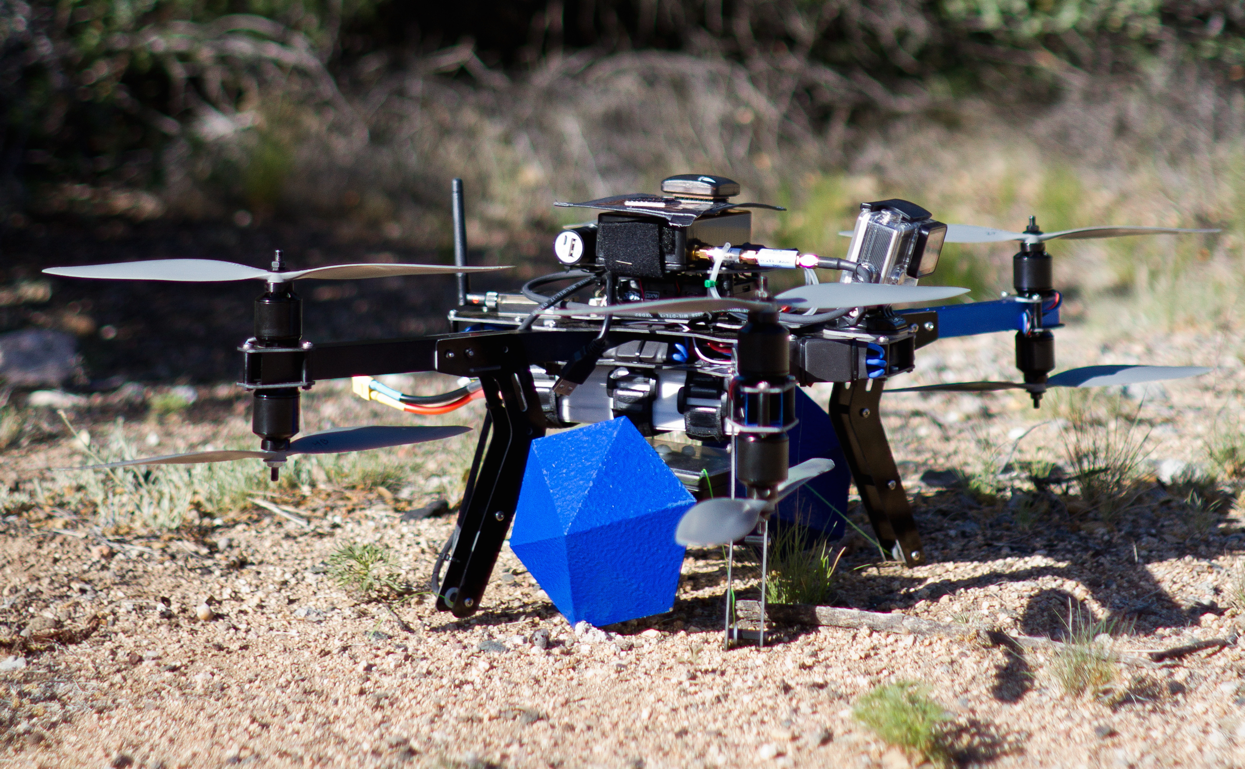
\includegraphics[width=0.59\textwidth]{figures/drone2.png}
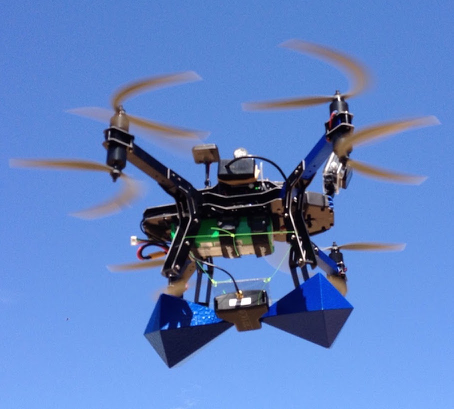
\includegraphics[width=0.4\textwidth]{figures/drone.png}
\caption{3DR X8 octoquad drone prior to launch (left) and in flight (right).  The transmitter is contained in the black project box mounted on top of the drone.  A copper plate, which acts as shielding from the electronics below, with the attached GPS magnetometer can be seen atop the project box. Beneath the drone, the blue  BicoLOG antenna is slung with non-conductive monofilament.}
\label{fig:drone}
\end{figure*}

Beam calibration of low frequency dipole arrays poses several complications compared to traditional dish antennas. Most notable is that traditional beam calibration, where the beam is scanned across a bright isolated source, is not possible because arrays are fixed to the earth. Phased array beams are technically steerable but violate the assumption that the beam is constant as it scans. Drift scan calibration of dipole array beams is possible --imaging point sources as they track across the beam--- but it requires the test antenna/array to be embedded within an existing array that generates sufficient sensitivity to isolate a large number of radio sources to provide many tracks through the beam. \citet{Pober:2013p9942} have employed symmetry arguments to reduce the needed number of sources on the sky and improve the result for PAPER antennas, but this is not possible in general for more complicated dipole array beam patterns and is ultimately limited by the symmetry argument and in the sensitivity far out in the beam.  Attempts have been made to use anechoic chambers to calibrate low-frequency phased arrays, but the measurements suffer since even the largest chambers cannot extend into the farfield pattern and the RF absorber material used in the chambers performs poorly below 150 MHz, creating reflections and resonances and in any case does not capture the as-built variation. Mapping beam response using the Orbcomm constellation of satellites has proven the most effective \citep{2015RaSc...50..614N,2016:NebenHERAdish} but is limited to only a single frequency (138 MHz).  

Drone-based radio calibration has recently been explored for application to widefield 21cm instruments.  A drone-mounted calibration source was used to verify the accuracy of antenna response modeling for SKA-low stations \cite{2014IAWPL..13..169V} and then a second generation setup was then used as a phase calibrator \citep{2015ExA....39..405P}.  Fully mapping the beam of an antenna has been demonstrated by \citet{2015PASP..127.1131C}.  In that experiment, a 5m dish was mapped at 1GHz with a noise source broadcast by a gimbal mounted horn. This experiment provided a first demonstration of the drone beam-mapping concept and identified places for improvement of the methods. 



Future improvement areas included: optimizing the flight path to better sample the beam, obtaining better drone positioning accuracy, improving characterization of the transmitter beam, and better modeling of the antenna under test. This last point was partially motivated by a lack of alternate beam mapping data with which to compare the results. Additional changes must be made in the shift from low redshift intensity mapping applications at 1GHz to reionization and cosmic dawn 200MHz.  At these lower frequencies horns and other highly directive elements become prohibitively large and heavy for flight applications, motivating the use of a fixed dipole, such as was used by \citet{2014IAWPL..13..169V}, while the broader effective bandwidths and heavier power amplifiers make coverage of the entire band add additional weight. The use of a fixed dipole puts further emphasis on the need to better understand the transmitter beam pattern with modeling and alternate measurements. 


Here in this paper we report our progress towards overcoming some of these challenges and describe the development of a system targeting the low frequency 21cm band and the requirements identified above.  In section \ref{sec:design} describe our own drone and transmitter design, improved flight procedure and analysis method.  In section \ref{sec:cal} we detail the results of mapping the reference dipoles used in the Orbcomm mapping setup which lets us compare with both detailed models and measured beam response maps.  Section \ref{sec:mwa} relates an initial trial measurement of an MWA tile. Section \ref{sec:conc} summarizes the results so far and outlines the next steps.


\begin{figure*}[htb]
\begin{center}
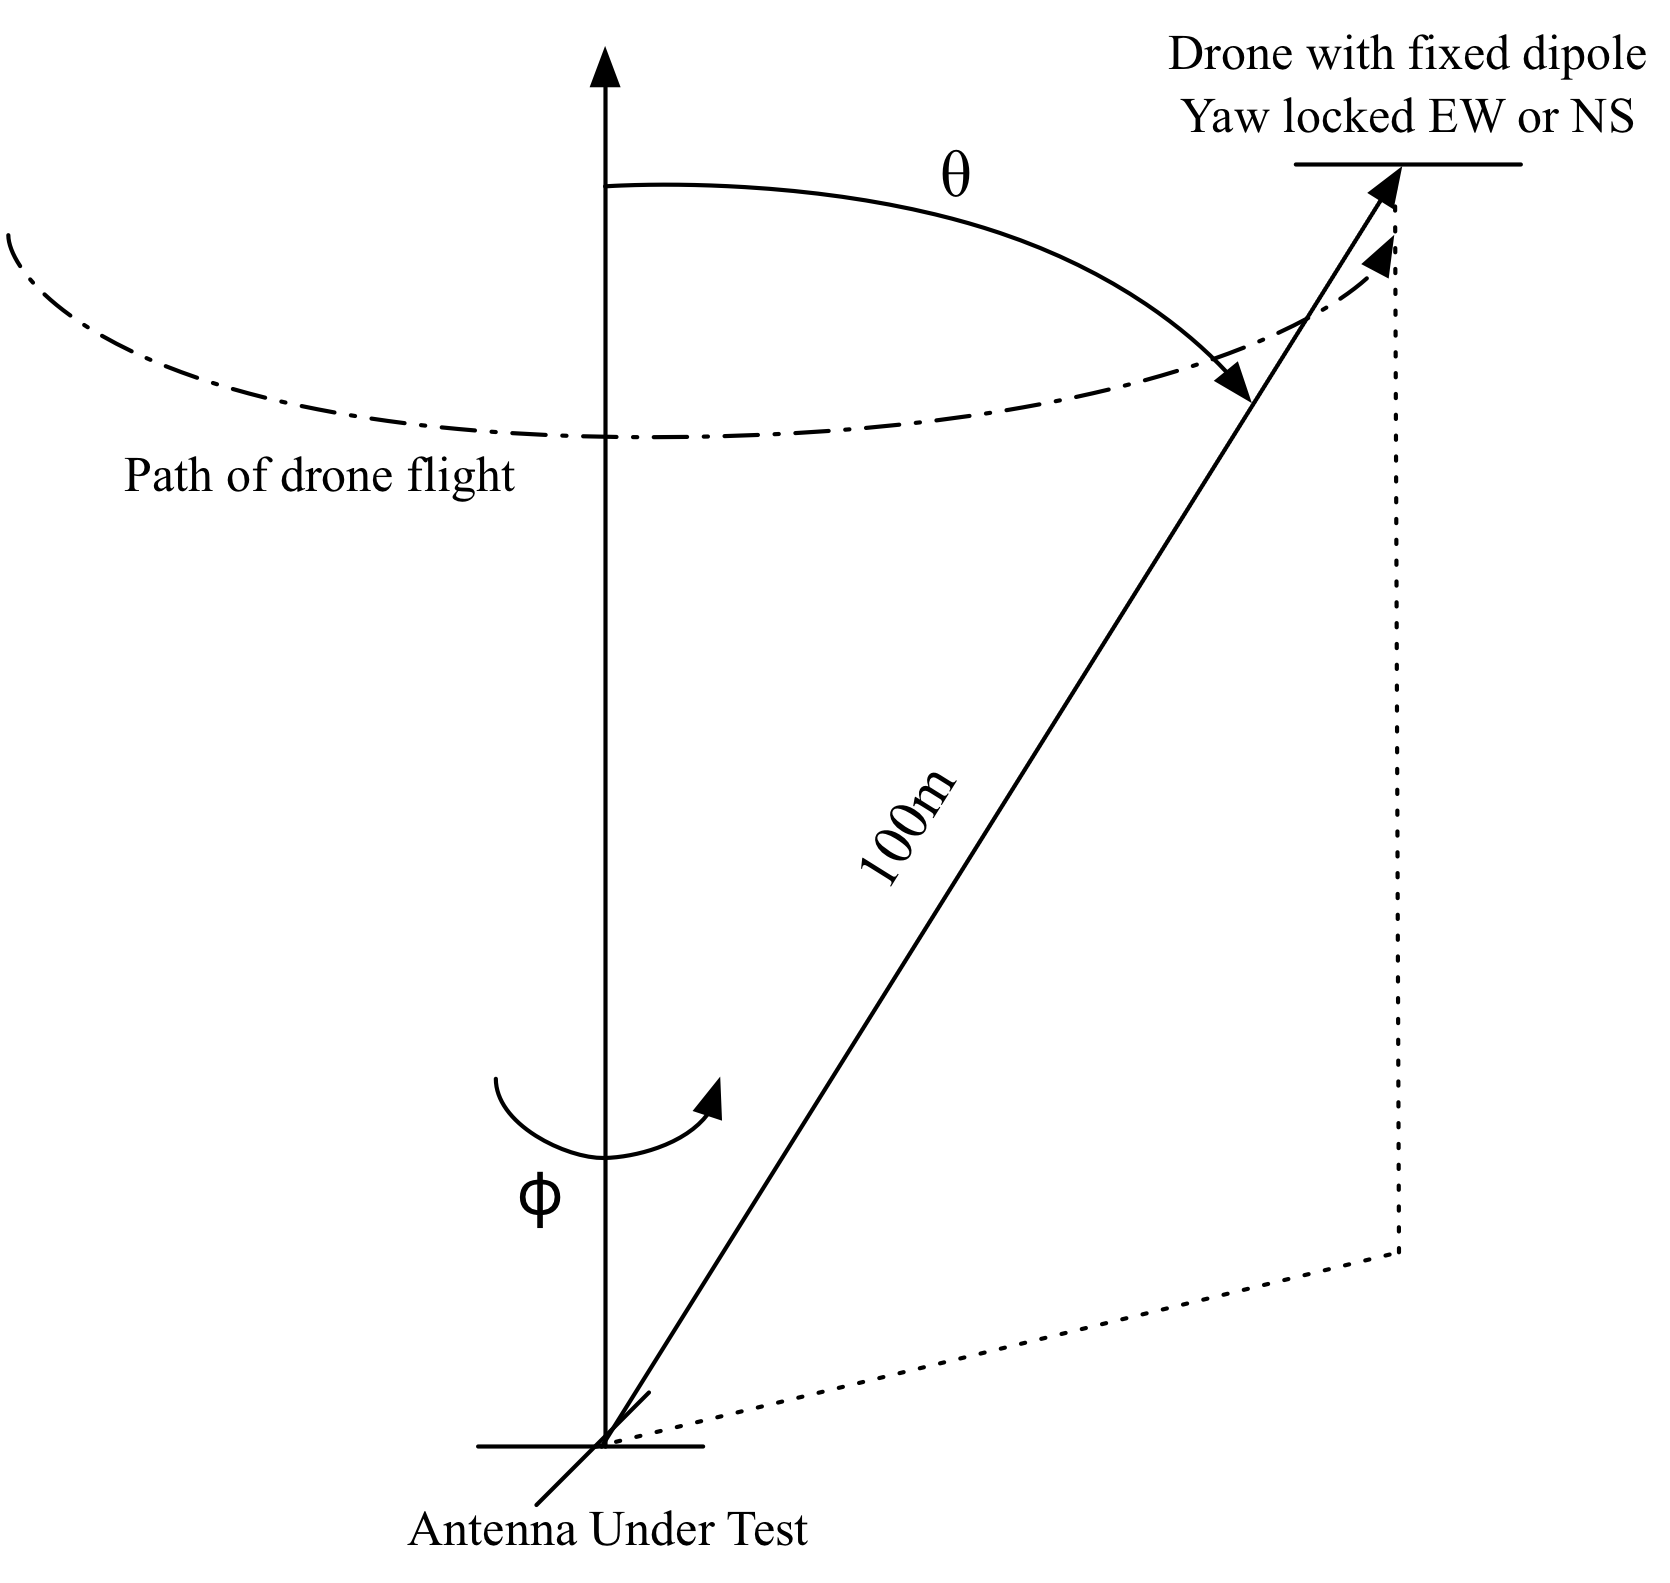
\includegraphics[width=0.6\columnwidth]{figures/ECHO_flight_diagram.png}
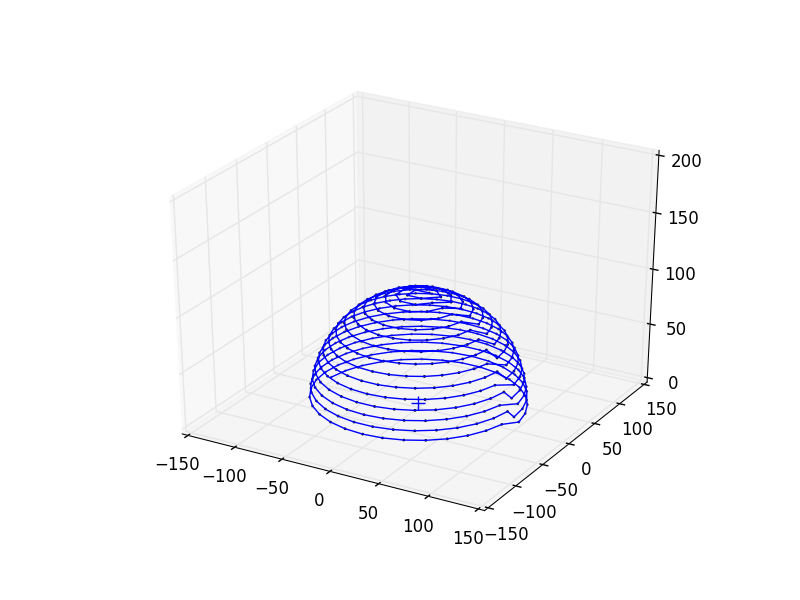
\includegraphics[width=0.39\textwidth]{figures/ECHO_flight_path.png}
\caption{The spherical coordinate system used here relative to the antenna under test (left) and the programmed flight pattern which uses the healpix equal area pixelization to form spherical shell of radius 100m centered on the antenna under test (right). In all flights the dipole antenna is mounted in a fixed position relative to the drone and the drone itself. }
\end{center}
\end{figure*}

\section{Design and Method}
\label{sec:design}

\subsection{Drone and Transmitter}
The drone is an X8 octoquad from 3DRobotics (3DR) with a Pixhawk autopilot running Arducopter 3.5.  With a 10,000 mAh battery and a 1kg payload this setup has a flight time of $\sim$15 minutes. Position is recorded by a ublox GPS and a barometric altimeter.  The transmitter is a programmable Valon 5007 voltage controlled oscillator. Typically used as a clock signal this device can produce a stable, continuous wave, signal tuned from 137\,MHz to 5\,GHz and is programmable via usb interface.  A continuous wave signal is chosen over a broadband signal for our first testing because the power is concentrated in a narrow band and does not require additional amplification. This reduces both weight and complexity and enables better flexibility to avoid interference.  In the work reported here the transmitter is programmed to broadcast at 137.5\,MHz with attenuation added to produce -25dBm of output power chosen to reach a peak SNR of 40dB without evidence of saturation in the receiver.  The transmit antenna is a BicoLOG 30100 biconical antenna manufactured by Aaronia. It is completely passive, has a smooth spectral response, an operational spectral range of 20\,MHz to 3\,GHz and is light-weight yet robust. 



\subsection{Antenna Mount}
The antenna mounting is chosen to maximize the distance from the drone while preserving stability. The X8 drone legs are too short to permit a fixed mounting further than two or three centimeters below the drone and the wingspan is too narrow for safe landing on longer legs. In the tests here the antenna has been suspended from the drone legs by non-conductive monofilament with a plastic bracket providing the filament/antenna mount point. On the ground, the antenna fits between the legs, in the air the antenna hangs 30\,cm below, this is shown in Figure \ref{fig:drone}. The advantages of this system are that it is simple, extremely light-weight and provides isolation between done and antenna. The disadvantages are that it lacks rigidity, stability, and because it must be re-tied after transport it is difficult to repeat.

\subsection{Flight Path}
One of the main difficulties encountered by \citet{2015PASP..127.1131C} was in matching the flight pattern to the size scale of the variation in the beam.  They chose a cartesian grid pattern with a separation such that the drone passed through the primary lobe roughly three times.  When combined with the on/off switching used to subtract the 1GHz noise of the drone motors, the number density of samples became extremely limited and led to spurious results when interpolating to make a complete beam map.  Here our goal is to smoothly map the beam of a very wide-field element from zenith to the horizon, which would be difficult with a constant altitude flight pattern.  This is also true of the analysis pipelines where the distortion caused by the gnomic projection to a tangent plane makes for a poor gridding scheme at the horizon. In many 21cm pipelines, the HEALPix pixelization scheme \citep{Gorski:2005p7667} is used to store images and beam models.  HEALPix divides the sky into equal area pixels with the pixel count and resolution increasing by powers of two.
\begin{equation}
N_{\mathrm{pix}} = 12 * \mathrm{Nside}^2
\end{equation}
Pixels can be ordered either by their position in the hierarchical doubling (NEST) or in a spiral order with  longitude $\phi$ fastest (RING).  Here we chose a flight pattern which follows the NEST pattern to give us spherical shell flight pattern centered on the AUT with chosen a radius. Following a conservative safety practice limiting to good line of sight and considering the FAA flight ceiling of 400 ft we set the radius (and thus the maximum altitude) to 100m (328ft). The NSIDE parameter sets the number of waypoints and, effectively, the resolution of the beam sampling.  This number is constrained, ultimately by the amount of time we're willing to spend getting a beam map; at constant speed, a denser grid will take longer to record.  The slowest variable to be sampled is GPS position at 2 Hz. We've chosen to fly at 1m/s where the drone will sample about 3 samples per angular degree and an NSIDE of 8.  At this resolution and speed the full $2\pi$ steradians can be mapped to a resolution of 9 degrees in 60 minutes with four 15 minute sorties.

The polarization of the antenna is kept fixed by inserting a Region of Interest (ROI) command into the beginning of the waypoint program.  The ROI command causes the drone to maintain a fixed heading in the direction of a set location which we choose to be a distant location due East or North as the required.

\subsection{Receiver}
Below we relate two experiments: mapping of calibration dipoles and a first map of an MWA tile. During the calibration experiment data was collected using the spectrometer setup of the Orbcomm satellite mapping array as described in section 2.4 of \citet{2016:NebenHERAdish}. The software was modified to allow real time inspection of the data, but otherwise the system was operated just as it was for satellite mapping with spectra recorded simultaneously from two dual polarization dipoles at a time cadence of 4 Hz and a spectral resolution of 2kHz. Data from the MWA tile was collected with a SignalHound software defined radio run in spectrometer mode with a spectral resolution of 5kHz and a time cadence of 2.22Hz. 
\subsection{Data processing}
We generate a beam map by interpolating the power trace at times when recorded GPS positions are available.  Careful observation of the autopilot behavior and inspection of logs suggests that the X8/Arducopter combination suffers from occasional stability `hiccups'. Finding that these are characterized primarily by outliers in the yaw we have flagged points greater than 2 $\sigma$ above the mean yaw.  Another slight yaw outlier is observed to occur as the drone passes through each waypoint gate which is often accompanied by a visible bump in the received power trace; points within half a second of each waypoint have been flagged (see Figure \ref{fig:waypoint_flagging}).

\begin{figure}[htb]
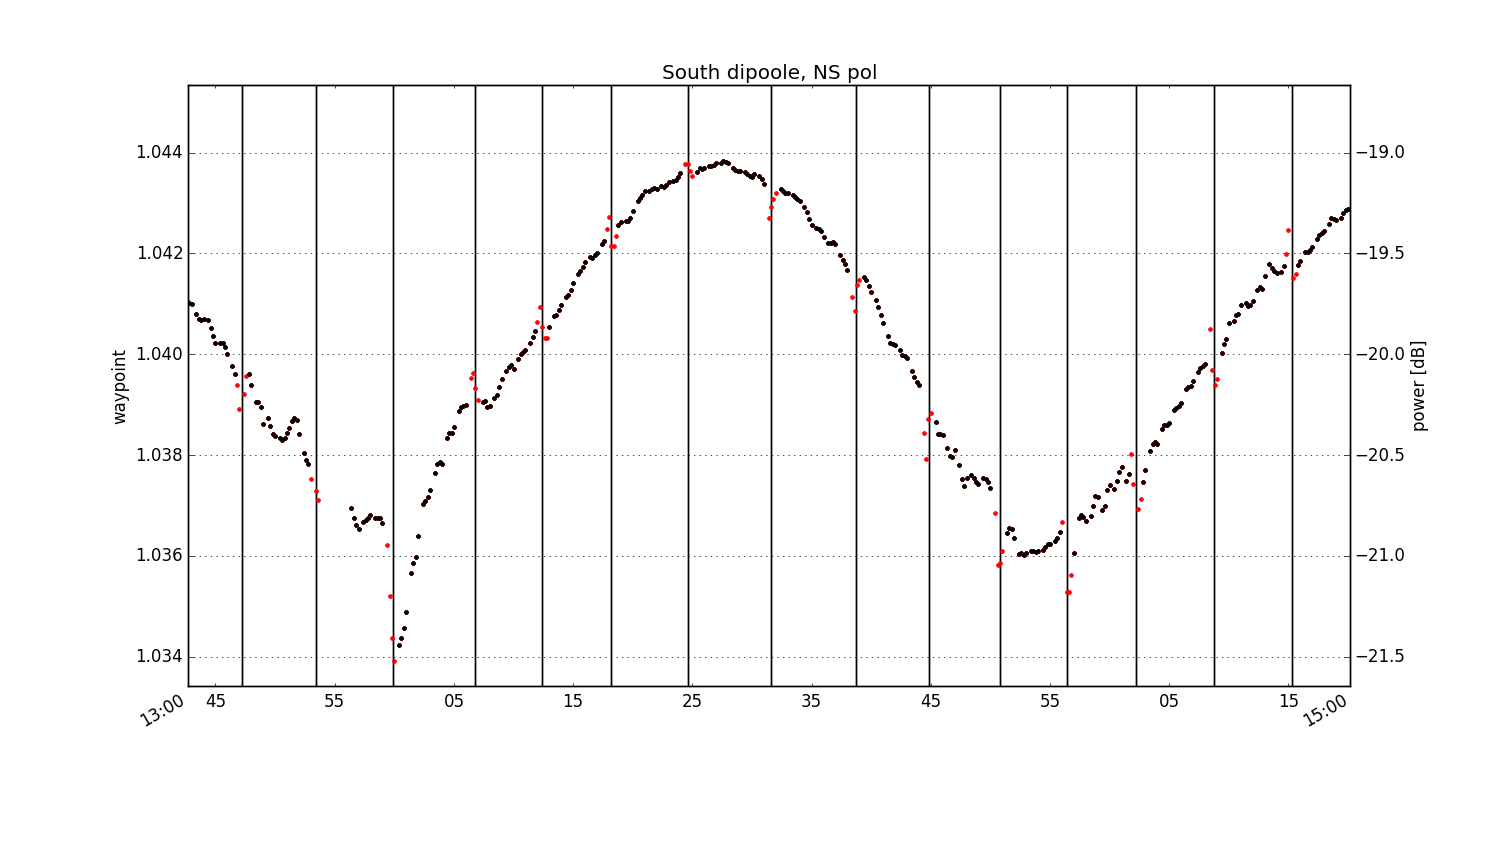
\includegraphics[width=\columnwidth]{figures/GB_waypoint_flagging_zoom.png}
\caption{The drone is observed to shudder slightly when it goes through waypoints (vertical lines) and it can be seen in the received power. Here we flag received data within half a second of a waypoint arrival.}
\label{fig:waypoint_flagging}
\end{figure}


These flagged data are then gridded, using a nearest pixel approach, into a healpix grid using an NSIDE of 8, the same as the flight pattern.  The gridder records the mean, the standard deviation and the total sample count of all the samples falling into each pixel. An example gridded beam is shown in Figure \ref{fig:beam_std_count}.

The measured power pattern is a product of the power patterns of the transmitter and receiver. To estimate the power pattern of the receiver we use CST Microwave Studio to model the transmitting bicolog antenna beneath the drone modeled as a set of metal arms (see Figure \ref{fig:tx_cst}).  


\begin{figure}
\caption{A view of the CST model of the transmitting antenna suspended beneath the metal arms of the drone.}\label{fig:tx_cst}
\end{figure}


\begin{figure*}[htb]
\begin{center}
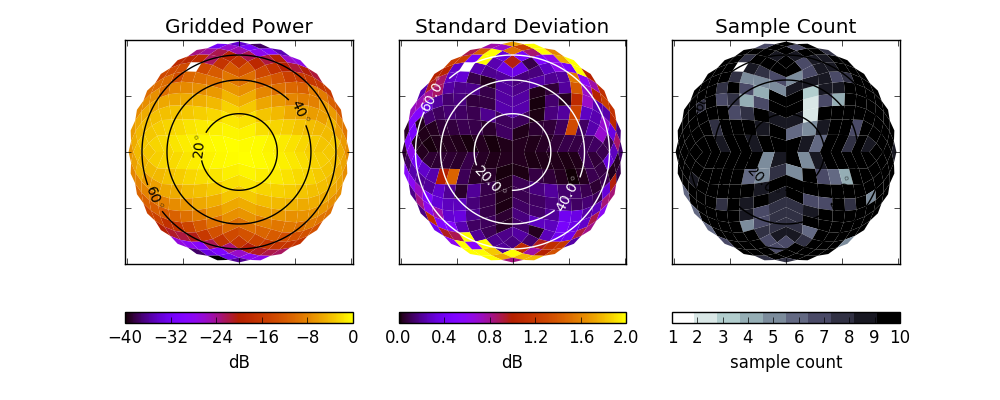
\includegraphics[width=\textwidth]{figures/GB_power_rms_count.png}
\caption{Received power pattern, error, and sample count for a calibration dipole.}
\label{fig:beam_std_count}
\end{center}
\end{figure*}

\section{Calibration}
As a first test of stability and accuracy we used ECHO to map antennas which had already been mapped using the Orbcomm satellite constellation .  The Orbcomm system measures the power received by multiple satellites, operating in narrow band channels at 137 MHz and uses the telemetry in those signals to associate the received channel powers with the orbital positions of the satellites.   The time variation of the digital signal is removed by simultaneously measuring the power received by the antenna under test (AUT) and a nearby sleeved dipole. The ratio between these two is insensitive to satellite transmitter variations; the dipole acts as a precision calibration element. The AUT beam is referenced to this standard dipole which is can be calibrated out using a model.  The accuracy and repeatability of the dipole established with a ``null'' test where the AUT is replaced with a second identical calibration dipole.  It was in this configuration that we performed the calibration test described here.

\begin{figure}
\begin{center}
\includegraphics[width=\columnwidth]{figures/Green_Bank_aerial_diagram.png}
\caption{An aerial view of the Orbcomm experimental setup in Green Bank. Each calibration dipole is a dual polarization linear feed mounted on a 2m x 2m mesh set $\sim$20cm above the ground. The spherical flight pattern is centered on each at a radius of 100m.}
\label{fig:GB_aerial}
\end{center}
\end{figure}


Data were collected in a series of four mapping runs in August, 2015 at the Green Bank Observatory operated by the National Radio Astronomy Observatory.  The amplifier and receiver setup was left unchanged from normal Orbcomm operations with the exception that the data recording script was modified to increase the spectral dump rate. The ECHO transmitter was tuned to 137.5\,MHz and attenuation was added until, at an output power of -22dBm, saturation into adjacent channels was no longer visible.  This resulted in a signal of amplitude similar to the received Orbcomm signals. Historical recordings were examined and this channel was seen to be rarely used by Orbcomm making an overlap unlikely.  The output was monitored throughout operations for obvious signs of an overlapping Orbcomm transmission.

The null experiment, shown in an aerial view in Figure \ref{fig:GB_aerial}, was set up with the antennas separated by 50m along a north-south line with a HERA dish at the north end.  Each station was mapped twice, once with the transmitter fixed in the east-west (EW) direction and once north-south (NS).

%The first full scale test of the ECHO system was done in August, 2015 at the National Radio Astronomy Observatory (NRAO) site in Green Bank, WV.  Two dual-polarization dipoles (see Fig.~\ref{fig:dual dipole}) used in the development of a calibration technique utilizing the ORBCOMM satellite constellation (Neben et al. 2015) were used as the AUTs.  With a dipole length of 90.4 cm and a Valon synth frequency of 137.5 MHz, a flight radius of 100m was chosen, well into the far-field of the dipoles.  Choosing a flight speed of 0.2 dam s$^{-1}$ and $N_{side}=8$, each flight ECHO performed took ~60 min.  Four total flights were performed as each antenna contained two dipoles and thus needed to be tested with two flights, one with a polarization of the BicoLOG matching the polarization of one of the dipoles.  This also allowed cross-polarization measurements of each antenna to be made.


\subsection{Maps}




\begin{figure}[htb]
\begin{center}
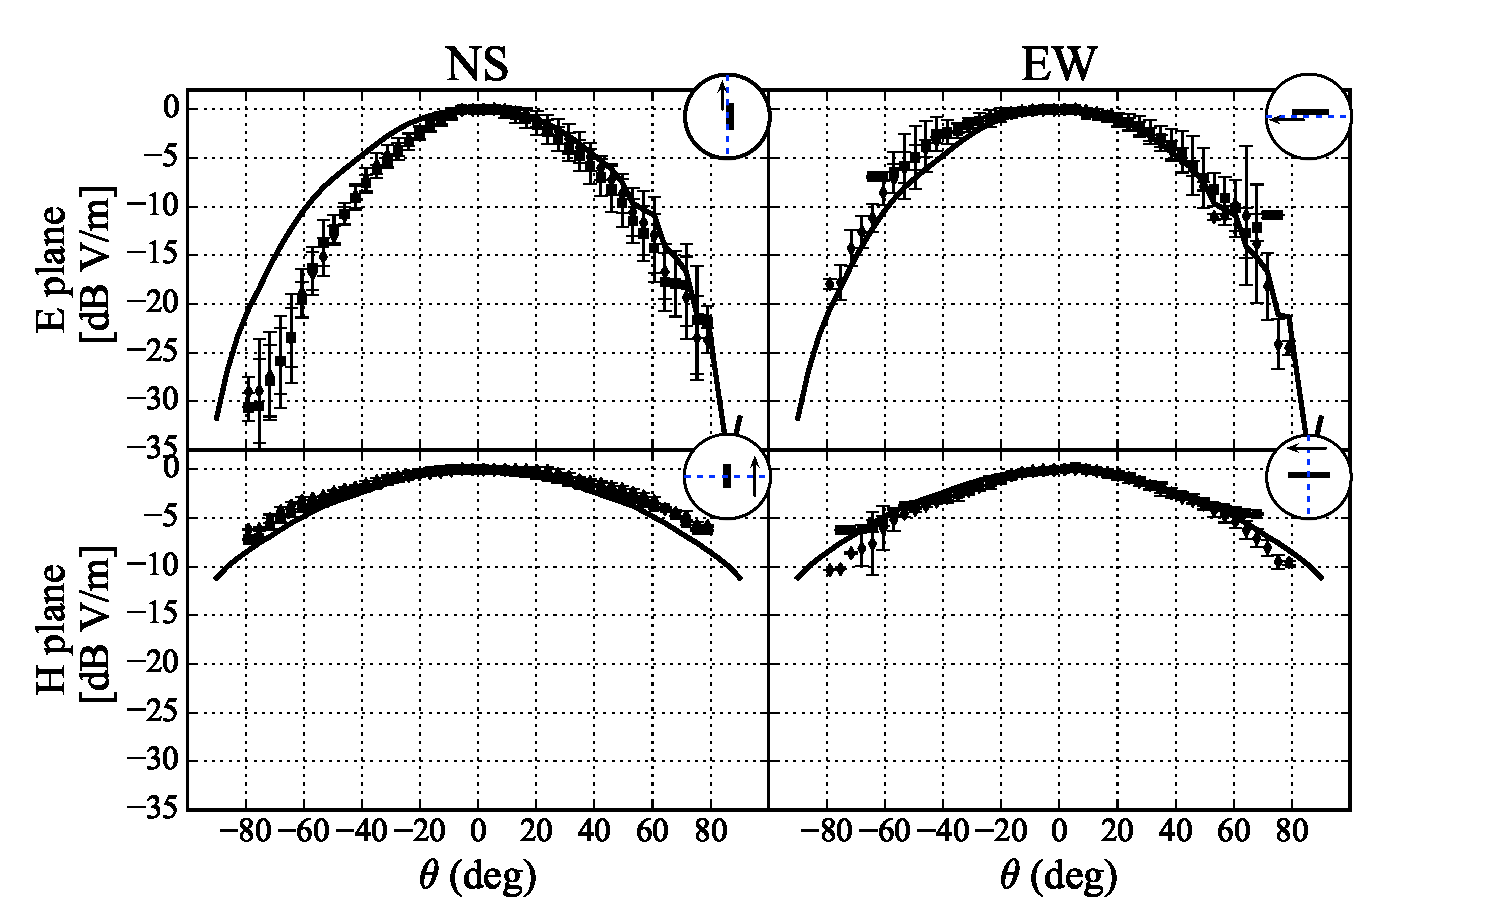
\includegraphics[width=\columnwidth]{figures/GB_slices_quad.png}
\caption{Slices of dipole maps after subtracting transmitter beam pattern. Two identical full linear polarization feeds were mapped.  Here we divide them up by polarization (NS vs EW) and by slice plane. The E plane is parallel to the dipole  and the H plane cuts E perpindicularly 90 degrees.  Antenna 'A' is square symbols, antenna 'B' is diamonds. }
\end{center}
\end{figure}

\subsection{Comparison to Orbcomm Ratio Maps}

\begin{figure}[htb]
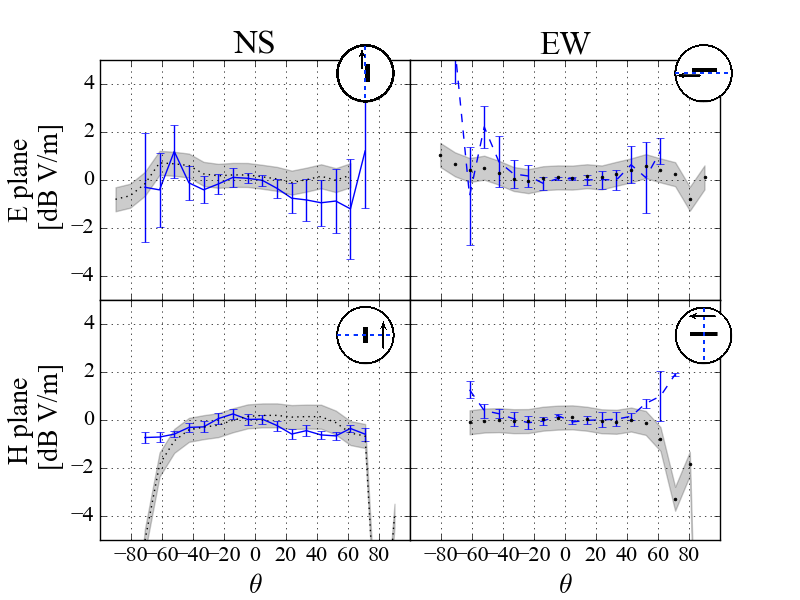
\includegraphics[width=\columnwidth]{figures/GB_ratio_slice_5dB.png}
\caption{Ratio of the two calibration dipoles.  }
\end{figure}


\section{MWA Tile}

\subsection{Data}
\begin{figure}[htb]
\includegraphics[width=\columnwidth]{figures/MWATile_slice.png}
\caption{MWA tile map compared with approximate model. Note that tile is surrounded by an 8 foot chain link fence which is not included in the model.}
\end{figure}
\subsection{Systematic Variation}

\subsection{Comparison to Orbcomm Maps}





\section{Conclusion}


\acknowledgments
ECHO development is supported by a grant from the National Science Foundation AST program, award number 1407646. D.C.J would like to acknowledge NSF support  under award 1401708.
Thanks to Rich Bradley and National Radio Astronomy Observatory, Green Bank and to Andri Gretarsson and Embry Riddle Aeronautical Observatory for generously supporting this project with their time and equipment.

\bibliographystyle{apj}
\bibliography{library}

\end{document}




